 %% Copyright (C) 2021 by
 %%   Robert L. Read <read.robert@gmail.com>, Megan Cadena <megancad@gmail.com>

 %% This program is free software: you can redistribute it and/or modify
 %% it under the terms of the GNU General Public License as published by
 %% the Free Software Foundation, either version 3 of the License, or
 %% (at your option) any later version.

 %% This program is distributed in the hope that it will be useful,
 %% but WITHOUT ANY WARRANTY; without even the implied warranty of
 %% MERCHANTABILITY or FITNESS FOR A PARTICULAR PURPOSE.  See the
 %% GNU General Public License for more details.

 %% You should have received a copy of the GNU General Public License
 %% along with this program.  If not, see <http://www.gnu.org/licenses/>.

\documentclass{article}
\usepackage[backend=biber]{biblatex}
\addbibresource{softrobotmath.bib}
\usepackage{hyperref}
\usepackage{amsmath}
\usepackage{amssymb}
\usepackage{mathtools}
\usepackage{draftwatermark}
\usepackage{listings}

\usepackage{flexisym}
\usepackage{breqn}
\breqnsetup{breakdepth={1}}


\SetWatermarkText{DRAFT}
\SetWatermarkScale{6}
\SetWatermarkLightness{0.95}

\title{Three Inflatable Spheres as a Theoretical Basis for a Parallel Manipulator}

\author{Robert L. Read
  \thanks{read.robert@gmail.com}
  email: \href{mailto:read.robert@gmail.com}{read.robert@gmail.com}\\
Megan Cadena
  \thanks{megancad@gmail.com}
  email: \href{mailto:megancad@gmail.com}{megancad@gmail.com}
  }


\begin{document}
A Stewart Platform\cite{wiki:stewart} is a fundamental mechanism for varying the angle

\maketitle
\begin{abstract}
  A Stewart Platform\cite{wiki:stewart} is a fundamental mechanism for varying the angle
  between two objects.
  A soft Stewart Platform can be made of two discs and
  three inflatable spheres.
  Stacking such devices might make a soft tentacle.
  Soft robots are meant to deform under force, but it is useful to have
  an analytic description of a plane in contact with three spheres
  before deforming force is applied.
  In 1881, the problem of computing the plane tangent to three spheres was
  set as an exercise in a textbook, {em Practical Solid Geometry}\cite{payne1881},
  but not solved.
  We have solved the problem of computing the plane in contact with
  three adjacent spheres from known radii via close-form expressions and
  in JavaScript, producing an interactive,
  browser-based web page that dynamically solves the problem\cite{softrobotcalc}.
  More importantly, we have solved the inverse problem, of computing the
  sphere radii which orient a plane in contact with all three spheres, in
  both closed-form solutions and on the web page.
  This would allow a soft Stewart Platform or a tentacle to be positioned
  in basis by choosing the expansion of inflatable spheres.
  The closed-form expressions allow derivatives and Jacobians to be computed
  symbolically.
  All of the code is released under the GNU Public License.
\end{abstract}


\section{Introduction}

A parallel manipulator varies the angle between two planes.
The best known parallel manipulator is
a Stewart Platform\cite{wiki:stewart} which as 6 degrees or freedom.
Having a soft parallel manipulator analogous to a Stewart Platform would allow soft,
gentle positioning,
and might be particularly valuable {\it in vivo}\cite{softwhite2018soft} or in some space applications\cite{glassner2020}.
Varying angular displacemnt is a composable buliding block of more complicated systems, such as tentacles.

One way theoretical way to build such a manipulator is to have three inflatable spheres sandwiched between two planes
and constrained to always be in contact with each other.
As these spheres are inflated or deflated changing
their size, the top plane changes its orientation relative to the bottom plane.
This creates a 3-degrees-of-rotation system
(ignoring the slight translation the spheres are capable of by consistently enlarging),
which is slightly more constrained than the 6DOF Stewart Platform.
This paper gives closed-form expressions of both
the forward and inverse problem as pure solid geometry.
The forward problem is given three radii,
to determine the orientation of the top plane.
The inverse problem is much harder: given a desired orientation and the radius of one
sphere, find the radius of the other two spheres that acheives it.

Additionally, we have create an online, browser based realtime simulation that reifies
the math in this paper in JavaScript, both verifying it and making it easy to reuse.

Soft robotics presume to operate under some deforming forces, so the precise mathematics
of positioning must always be corrected by a control system with feedback on the position.
Nonetheless, having a closed-form expression of both the inverse and forward problem allow
an initial Jacobian to be computed effortlessly, which is likely to assist any control algorithm.

\section{The Center Plane}

As kinematicists,
our interest is in the slope of the plane of the tops of these spheres
as if they were resting on a fixed-frame such as a table. Then by inflating or deflating spheres,
we would be able to control the direction of the top plane or platform.

Choosing the coordinate system of the $XZ$ plane through the center of the spheres greatly
simplifies the derivations, because the center of the spheres always form tangent circles
in this plane. Call this plane the {\em center plane.}
Following computer graphics convention, we think of the $Y$ dimension as vertical and a
right-handed set of axes.
The position of $A$ is fixed at the origin, $B$ is constrained to the $x$-axis touching $A$, and
$C$ is contrained to the positive $xz$-plane. The center of these circles in the $xz$ plane can be
calculated from the radii independent of the tilt they induce.
In this coordinate system, the $y$-coordinate of the center of all spheres is $0$.
Furthermore, a cone tangent to two spheres has its axis and apex in the $xz$-plane.
The projection of all three spheres into this plane produces three touching circles.
We seek an expression for the normal of the plane of the tops of these spheres as a function
purely of the three radii. Call this plane the {\em top plane}.
We can imagine the spheres resting on a fixed surface called the {\em bottom plane}.
The tilt of the top and bottom plane relative to the center of the spheres
is alway a mirror image of each other across the coordinate $XZ$-plane.


Define extrinsic Euler angles $\theta$ to be the rotation about the $Z$-axis and then $\gamma$ to
be the rotaion about the $X$-axis.
The tilt of the top plane relative
to the bottom plane is given by the $zx$ extrinsic Euler angles $(2\theta, 2\gamma)$.\footnote{Is this really true?
We should be able to verify this with a JavaScript program.}

Because there is a plane through any three points and we have three spheres, we can construct the plane through
the center of these points.
The projection of the edges of the spheres onto this plane form three touching circles.

\begin{figure}
     \centering
     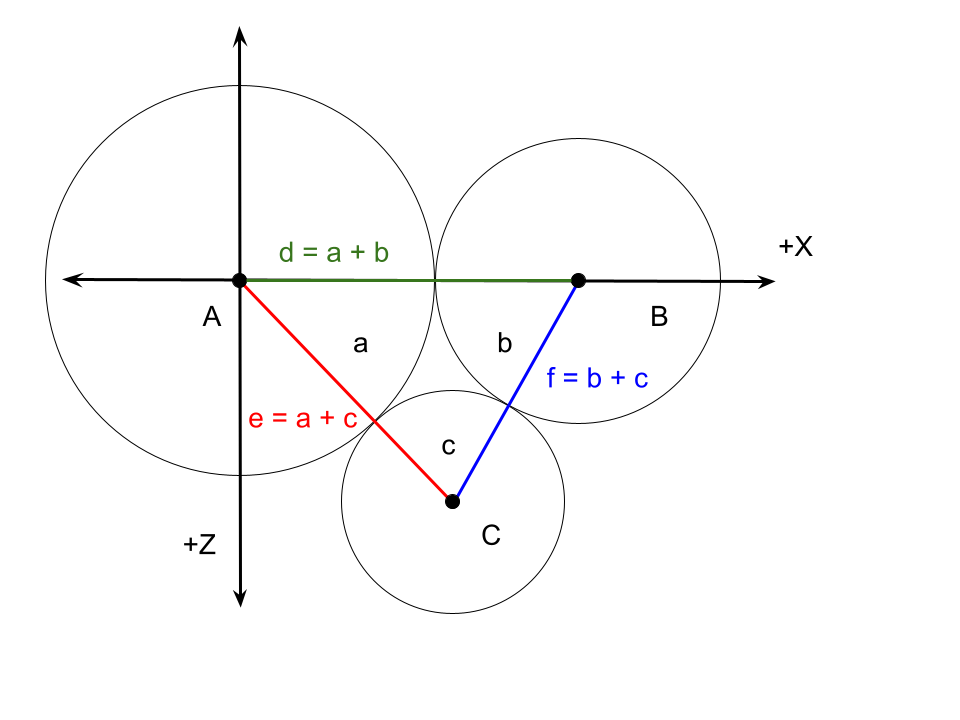
\includegraphics[width=0.8\textwidth]{figures/ThreeTouchingPlanarCircles.png}
     \caption{Three Touching Circles}
  \label{fig:Tangent}
\end{figure}

To solve this problem most conveniently, we place the first circle at the orign, and the second circle
on the positive $x$-axis, with the circles intersecting at the origin.
The third circle is place in the positive $z$ direction touching both other circles.

We seek a formula for the coordinates of the third circle in terms of three input radii $a,b,c$.

Because the distance between adjacent circles is the sum of their radii, define:
\begin{align}
  d  &= a + b \\
  e  &= a + c \\
  f  &= b + c \\
\end{align}

\section{The Tilt from the Radii}

Given $a,b$ and $c$, we seek the angles $\theta$ and $\gamma$.
We seek the  point $C$ first.
The cosine law to compute the angle $\angle ABC = \alpha$:

\begin{align}
  \alpha  &= \arccos{\frac{a^2 + b^2 - c^2}{2bc}} \\
%  \alpha  &= \arccos{\frac{(b+c)^2 + (a+c)^2 - (a+b)^2}{2(a+c)(a+b)}} \\
\end{align}

It is clear that once $\alpha$ has been calculated:

\begin{align}
 C_z  &= a\sin{\alpha}
\end{align}
Allowing us to form a right triangle $\triangle ACD$ and use the Pythagorean theorem:
\begin{align}
  C_x   &= \sqrt{b^2 - C_z^2}  \\
\end{align}



\begin{figure}
     \centering
     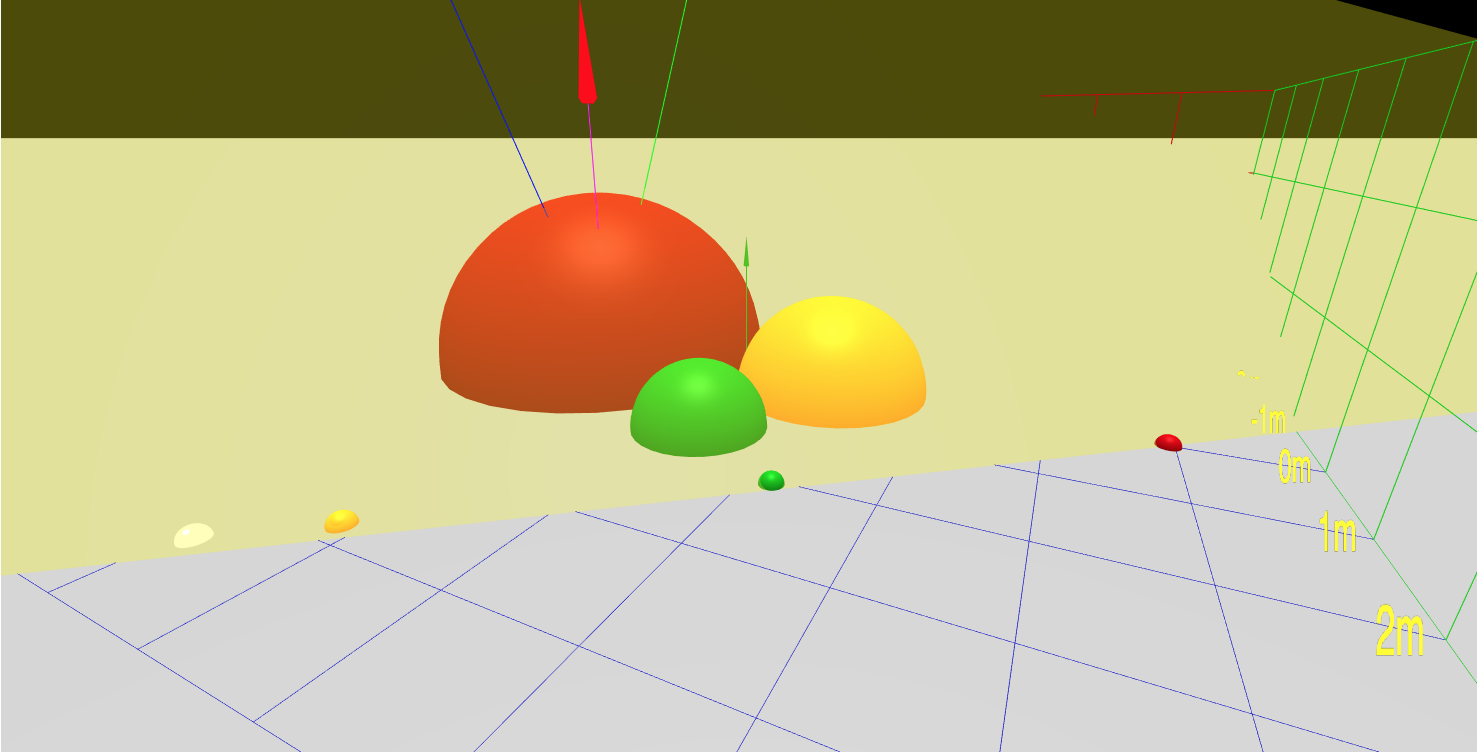
\includegraphics[width=0.99\textwidth]{figures/StandardThreeSphereDiagram.png}
     \caption{Three Touching Spheres}
  \label{fig:fixed}
\end{figure}


\subsection{Axis Angle of Cone Enveloping Two Spheres}

The problem of finding the planes tangent to three touching spheres
is given as an exercise in an advanaced textbook on solid geometry from 1881\cite{payne1881} which does not give a solution,
but it gives a hint: to consider the cones enveloping
three spheres taken two at a time.

Taking two adjacent spheres defines a cone tangent to both spheres whose apex is in the $XZ$ plane.
Call the apex of the $AB$ cone $U$, the $AC$ cone $V$, and the $BC$ cone $W$.

It is a beautiful fact that the the apices $U,V$ and $W$ are colinear
on the {\em apex line} which is in the $XZ$ plane, depicted in both Figure \ref{fig:fixed}
or Figure \ref{fig:rotation}.
Finally, the top and bottom planes
intersect at this line, because those planes are tangent to the three cones.

The apex angle $\psi$ of a cone which envelopes (by being tangent to) two tangent
spheres of radii $r,s$, is:

\begin{align}
 \psi &= \arcsin{\frac{s - r}{s + r}} \\
\end{align}
where $r < s$ without loss of generality. Note that when $r = s$
there is a special case,
the cone tangent to both is degenerate (that is, a cylinder, or a cone of
$\psi = 0$ apex angle.)

\subsection{Strategy}

We seek to compute the normal of the tangent plane.
Observe that this plane is tangent to all three cones.
Observe that the $AB$ cone intersects
the $A$ sphere in a circle on the surface of the $A$ perpendicular to and centered on the $X$ axis.

The half-angle of a cone tangent to two tangent spheres is computed from the radii directly:
\begin{align}
  \theta &= \arcsin{\frac{a - b}{a + b}} \label{eq:theta}\\
  \phi &= \arcsin{\frac{b - c}{b + c}}
\end{align}

\begin{figure}
     \centering
     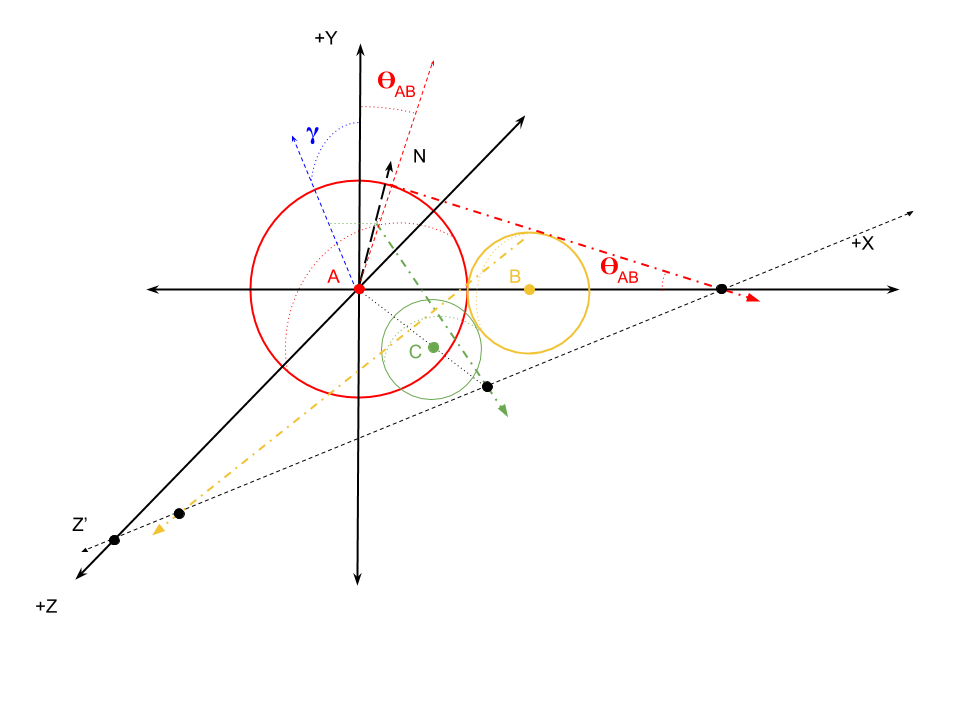
\includegraphics[width=0.9\textwidth]{figures/RotationMath.png}
     \caption{Rotation Math}
  \label{fig:rotation}
\end{figure}

A vector of length $a$ that is always rotated about the origin is always a point on the sphere.
The first operation is to move this vector perpendicular to the $AB$ cone.
A vector $N$ in the $Y$ direction and rotated counterclockwise
about the $Z$-axis by $\theta$ is perpendicular to the $AB$ cone.

However, we must rotate this vector $N$ about the $X$ axis by an unknown amount, $\gamma$, in order
to orient the vector to line up properly with the
desired tilt of the tangent plane despite not being a pure rotation about the $Z$ axis.
Since this angle is computed in the $YZ$ plane, we compute a projection of the point $V$ into
that plane, forming a triangle in the $YZ$ plane.

Call this point $I_z$, the intersection
of the apex line with the $Z$-axis. Let $h$ be the height of the intersection of the y-axis with the $AB$ cone.
Then $\gamma$ is the angle we need to rotate the plane by so that it intersects with the
$Z$-axis at a point, referred to as $Z'$.
By basic geometry of simialr triangles, this is computed from the right triangle of the origin with $h$ and $I_z$.
Points $U, V, $ and $W$ represent the apices of the apices of the cones tangent to $A$ and $B$, $B$ and $C$,
and $C$ and $A$ respectively. Recall that $A = [0,0,0]$.

\begin{align}
  U &= A + \overrightarrow{AB} \frac{a}{\sin{\theta}} \\
  V &= B + \overrightarrow{BC} \frac{b}{\sin{\phi}}
\end{align}
So long as $a \neq b$,
\begin{align}
  Z' &= \frac{U_z V_x}{U_x - V_x}, \text{if  $a \neq b$} \label{eq:zprime} \\
  Z' &= V_z, \text{if $a = b$}
\end{align}

The point $H$ is the intesection of the $AB$ cone with the $y$ axis.
\begin{align}
  H_y &= U_x \tan{\theta} \\
\end{align}
This is right triangle of the origin with the points $U$ and $H$. (The hypotenuse
of this triangle is $\overline{HU}$, and side adjacent to $\theta$ is $\overline{AU}$.)
It is computed by projecting the contact point of the top plane in the $xy$-plane
onto the $xz$-plane. This allows $\gamma$ to be computed as a pure rotation
about the $x$-axis.

\begin{align}
  \gamma &= \arcsin{\frac{Z'}{H_y}} \label{eq:gamma}
\end{align}

Equations \ref{eq:theta} and \ref{eq:gamma} give the Euler angles
$\theta$ and $\gamma$
for the tilt of the
tangent plane as a function of the three radii $a,b,c$.


\section{The Inverse Problem}

To build a useful robotic platform in by controlling the radii of the
spheres by inflating and deflating them, we wish to solve the inverse
problem. That is, given input $\theta$ and $\gamma$ as desired Euler
angles, we want to compute $a,b,c$ which acheive these angles.

Since these are smooth functions, the problem could be solved
easily by a Newton-Raphson style solver based on \ref{eq:theta} and \ref{eq:gamma}.
However, a closed-form solution is always superior, and allows derivatives,
and hence Jacobians, to be expressed symbolically as closed-form solutions.

The radius $b$ can be computed directly from $\theta$
because of our choice of coordinates.
By considering to proportionality of the similar triangles formed
by the contacts points of sphere $A$ and $B$ and their centers with $U_x$ in the $XY$ plane,
we obtain:
\begin{align}
  U_x &= \frac{a}{\sin{\theta}} \\
  b &= \frac{(U_x - a)\sin{\theta}}{\sin{\theta}+1}
\end{align}

\newcommand{\abs}[1]{ \left\lvert#1\right\rvert}

Given the plane defined by a known radius $a$, $\theta$ and $\gamma$,
the point $C$ is constrained by asserting that the perpendicular
distance to this plane of $C$ is $c$.
Additionally, in the central plane we have two other constraints,
that $C$ is placed so that it touches the circle centered on $A$ and
the circle centered on $B$.

Then we know that the point $C$ but have distance $a+c$ from
the point $A$ (the origin) and distance $b+c$ from the known
point $B$. These two constraints can be generated from the Pythagorean Theorem and can be expressed:
\begin{align}
a + c &= \sqrt{C_x^2 + C_z ^2} \label{eq:a_constraint}\\
b + c &= \sqrt{(a+b-C_x)^2 + C_z^2} \label{eq:b_constraint}
\end{align}

If we were to plot the point $C$ as $c$ increases, we
would find a gentle curve moving away from the intersection
of the circle $A$ and $B$. An additional constraint will
allow us to select a point on this curve.

This gives us three equations, which
should be more than enough to solve for the point $C$.

Let $H = [0, H_y,0]$.

Let $N$ be the normal to the plane (pointing up in our diagram
when $ a >= b >= c $.)

\begin{align}
\overrightarrow{N} &= \overrightarrow{Z' - U}  \times \overrightarrow{Z' - H}
\end{align}

Since we have the normal of the plane three points ($U,Z,H_y$) in the plane,
computing the distance from the point $C$ to the plane has a simple
formula.
We'll use the point $U = [Ux, 0, 0]$ as our main point.
In our situation, because the sphere $A$ is at the origin,
the equation of the top plane  is
$ \overrightarrow{N} \cdot \overrightarrow{U} = a$.
\begin{align}
a &= \frac{N \cdot U}{N_y} \\
c &= \frac{\abs{N \cdot P - a}}{\abs{N}} \\
c &= \frac{\abs{C_x  N_x  + C_z  N_z - a}}{1} \label{eq:c_constraint}
\end{align}

By substituting \ref{eq:c_constraint} into equations
\ref{eq:a_constraint} and \ref{eq:b_constraint},
we obtain:
\begin{align}
  a + \abs{C_x N_x + C_z N_z - a} &= \sqrt{C_x^2 + C_z^2} \\
  b + \abs{C_x N_x + C_z N_z - a} &= \sqrt{(a+b-C_x)^2 + C_z^2}
\end{align}

If the interior expression $C_x N_x + C_z N_z - a$ is positive,
then upon solving the system we find only imaginary solutions.

So assuming it is negative, we obtain:
\begin{align}
  2a + -C_x N_x + -C_z N_z  &= \sqrt{C_x^2 + C_z ^2} \\
  2b + -C_x N_x + -C_z N_z  &= \sqrt{(a+b-C_x)^2 + C_z^2}
\end{align}



This is a system of two nonlinear equations with unkowns $C_x$ and $C_z$.
Solving this system is beyond the capacities of the authors,
but not Mathematica, although the answer that Mathematica produces
in its raw form is half a page long.
Furthermore, there are actually two solutions, corresponding
to the two sides of the $AB$ line which the circle $C$ could be
on and satsify these constratints.
We have selected the solution that place $C$ in the positive $Z$
direction conformant to our problem set-up.

However, by introducing new variables to represent repeated
portions of this long expression, the expressions be
made tractable and easily programmed.

\begin{align}
M &= (a + b + a N_x - b N_x)^2 - 4 a b N_z^2 \\
L &= a (a + b + a N_x - b N_x) - b (a + b) N_z^2 \\
G &= -a^2 (a - b)^2 b N_z^2 \\
H &= 2 a (-1 + N_x) - b ((-1 + N_x)^2 + N_z^2) \\
F &= \sqrt{G H} \\
K &= 4 a^2 b^2 N_z^2 + 2 a^3 b (-3 + N_x) N_z^2 \\
J &= b^3 (-1 + N_x) N_z^2 \\
C_{x0} &= \frac{2 (F + a L)}{M} \\
C_{z0} &= \frac{K + 2 b F (-1 + N_x) -
  2 a (F (1 + N_x) + b^3 (-1 + N_x) N_z^2)}
{(a -  b) M N_z} \\
C_{x1} &= \frac{-2 F + 2 a L}{M} \\
  C_{z1} &= \frac{K - 2 b F (-1 + N_x) +
    2 a (F (1 + N_x) - b^3 (-1 + N_x) N_z^2)}
  {(a - b) M N_z}
\end{align}

One solution ($(C_{x0},C_{z0})$ or $(C_{x1},C_{z1})$) will be on the
positive side of the $X$ axis, but which one is highly dependendent
on the input variables, so both are computed and the positive $z$
value selected.

The variable $c$ can be compute from $a$, $C_x$ and $C_z$
form Eq. \ref{eq:a_constraint}.

This math can be found in the JavaScript which is licensed
under the GPL\cite{gplv3} at our website\cite{softrobotcalc}.

\section{Special case when }

In the above math when $\gamma$ is $0$, then $N_z$ is zero,
creating a division by zero.
In this case we can use the proportionality of similar
triangles to assert:
\begin{align}
  a &= c + \frac{a C_x}{U_x}
\end{align}
Combined with our previous equations
Eqn. \ref{eq:a_constraint} and Eqn. \ref{eq:b_constraint} in the plane
relating $C_x$ and $C_z$ to $c$,
we obtain the following equation:
\begin{align}
c & = \frac{a (a + b) (a - U_x)}{a^2 - a b + a U_x + b U_x}
\end{align}


\section{Special case when }

When $\theta = 0$, the point $U$ is at infinity or
cannot be found. In thise case $b = a$.
In this case the sphere $C$ is symmetrically
positioned in contact with $A$ and $B$ because
they have the same radius; therefore $x = a$ and:
\begin{align}
(a + c)^2 &= a^2 + z^2
\end{align}

In this case,
\begin{align}
Z' &= \frac{a}{\sin{\gamma}}
\end{align}

Projecting out the $X$ dimension and forming
similar triangles in the $YZ$ plane, we find that
\begin{align}
  \frac{a}{Z'} &= \frac{c}{Z'-z} \\
  c &= \frac{a( Z' -z )}{Z'} \label{eqn:cthetazero}
\end{align}

Asking Mathematica to solve these two non-linear equations, we obtain,
after again discarding the solution producing negative $z$ values:
\begin{align}
 z &=  \frac{2 a^2 Z' - \sqrt{a^4 (Z')^2 + 3 a^2 (Z')^4}}{a^2 - (Z')^2},
\end{align}
which allows us to obtain obtain $c$ from \ref{eqn:cthetazero}.

When both $\theta = 0$ and $\gamma = 0$, then $c = b = a$.

\section{Usage}

These equations can be used to compute the radii $b$ and $c$
from a given radius $a$ and either a desired normal or euler
angles. When implemented as a soft robot, it must be understand
that the center plane is conceptual. The roboticists probably
want to think of moving the top plane relative to the bottom plane,
which can be implemented as a simple rigid disc.
The angles and normals between the top and bottom and will be
twice the angles\footnote{Megan, is this really true? Can we simply double the angles? I think so, but that might not be true.} measured against the center plane.

Furthermore, an implementation based on soft inflatable spheres
will not be really acheive perfect spheres at any pressure.
Nonetheless, because these equations are trivial to implement
in a micro-controller, they make a good basis for a control
algorithm because it allows the Jacobian to be expressed as a
closed from solution. A Stewart platform implemented in this would
be expected to be have ``softly'' in response to pressure,
and yet have a predictable shape in the absence of external
forces.

A series of such Stewart platforms stacked together would make
a soft tentacle.

Note: These closed-form expressions make it possible to compute the Jacobian of the system (the change in in the position
of the plane relative to a change in the radius of any or all spheres.)

\printbibliography


\end{document}
